\subsection{Cálculo variacional}
\label{ssec:variational_calculus}

Seja $\mathcal{F}(q_1(t), \ldots, q_n(t), \dot q_1(t), \ldots, \dot q_n(t)) :=
\int_{t_0}^{t_1} \dif t~f(t, q_1(t), \ldots, q_n(t), \dot q_1(t), \ldots, \dot
q_n(t))$  um funcional que possua mínimos locais nas funções $\mathcal{Q} :=
\left\{\chi_1(t), \ldots, \chi_n(t) \right\}$. Então, $\forall i \in \{1,
\ldots,  n\}$, $\mathcal{Q}$ é a solução do sistema de equações diferenciais:

\begin{equation}
    \label{eq:lagrange}
    \dod{}{t} \del{ \dpd{f}{\dot q_i} } = \dpd{f}{q_i}
\end{equation}

\begin{eg}[Princípio de Fermat]
    \label{eg:fermat}
    O princípio de Fermat diz que a luz andando num meio percorre o caminho que
    minimiza o \textbf{tempo} de percurso. Isto é, dado um meio bidimensional
    cujo índice de refração depende da posição ($n = n(x,y)$), temos:

    \begin{equation}
        \begin{aligned}
        T = \int_{t_0}^{t_1} \dif t =&  \\
        = \frac{1}{c} \int_{t_0}^{t_1} \dif t~\frac{c}{v} \dod{s}{t} =& \\
        = \frac{1}{c} \int_{A}^{B} \dif s~n(x,y)  =& \\
        = \frac{1}{c} \int_{A}^{B} \sqrt{{\dif x}^2 + {\dif y}^2} n(x,y) =& \\
        = \frac{1}{c} \int_{x_0}^{x_1} \dif x \sqrt{1 + {\dot y}^2} ~ n(x,y) 
        \end{aligned}
    \end{equation}

    Onde $\dot y := \tod{y}{x}$. Desse modo, se definirmos o funcional
    $\mathcal{T}(y, \dot y) := \int_{x_0}^{x_1} \dif x \sqrt{1 + {\dot y}^2} ~
    n(x,y)$,  sabemos que o caminho $y(x)$ é solução da \autoref{eq:lagrange}
    para $f(x, y, \dot y) = \sqrt{1 + {\dot y}^2}~n(x,y)$.
\end{eg}


\begin{eg}[Catenária]
    \label{eg:catenaria}
    A catenária é a curva que minimiza a energia potencial gravitacional de uma
    corda inelástica presa pelas suas duas extremidades, e cujo corpo é livre e
    não encosta no chão.

    A energia potencial gravitacional de uma partícula puntiforme é dada por
    $E_g = mgy$, e, considerando uma corda com densidade linear de massa $\rho$,
    podemos fazer:

    \begin{equation}
        \begin{aligned}
            E_g = \int_M \dif m ~ gy =& \\
            = \int_A^B \dif s~\rho gy =& \\
            = \rho g \int_A^B \sqrt{{\dif x}^2 + {\dif y}^2}~y =& \\
            = \rho g \int_{x_0}^{x_1} \dif x~y \sqrt{1 + {\dot y}^2}
        \end{aligned}
    \end{equation}

    Novamente, $\dot y := \tod{y}{x}$. Também de forma análoga ao
    \autoref{eg:fermat}, definindo o funcional $\mathcal{E}(y, \dot y) :=
    \int_{x_0}^{x_1} \dif x~y \sqrt{1 + {\dot y}^2}$, teremos que a curva $y(x)$
    será a catenária, e será solução da \autoref{eq:lagrange} para $f(y, \dot y)
    = y \sqrt{1 + {\dot y}^2}$.
\end{eg}

Entre outros exemplos úteis, temos:

\begin{table}[H]
    \centering
    \begin{tabularx}{\textwidth}{lXr}
        \toprule
        Nome & Definição & Equação \\
        \midrule
        Braquistócrona & %
            Superfície que minimiza o tempo que uma partícula demora para %
            cair diagonalmente sob influência de um campo gravitacional & %
            $f(y, \dot y) = y^{\frac{1}{2}}~\sqrt{1 + {\dot y}^2}$ \\ 
        Geodésica hiperbólica & %
            Menor caminho entre dois pontos em um semiplano hiperbólico & %
            $f(y, \dot y) = y^{-1}~\sqrt{1 + {\dot y}^2}$ \\
        \bottomrule
    \end{tabularx}
    \caption{Resultados comuns de cálculos variacionais}
    \label{tab:varcalc_eg}
\end{table}

Essas equações podem ser derivadas de maneira extremamente similar à do
\autoref{eg:fermat} e do \autoref{eg:catenaria}. 

De maneira geral, se um funcional tem um lagrangiano $L$ (i.e. $\mathcal{F}=\int
\dif t~L$) independente da variável de integração (no caso, o tempo), pode-se
usar a Identidade de Beltrami para encontrar grandezas constantes que auxiliam
a resolução das equações de Euler-Lagrange:

\begin{namedeq}[Identidade de Beltrami]
    $\forall i \in \{1, \ldots, n\} \exists C_i = L - \dot q_i \tpd{L}{\dot
    q_i} \text{t.q.} \tod{C_i}{t} = 0$, i.e.:
    \begin{equation*}
        \label{eq:beltrami}
        \dod{}{t} \del{L - \dot q_i \dpd{L}{\dot q_i}} = 0, \forall i \in \{1, 
        \ldots, n\}
    \end{equation*}
\end{namedeq}

\subsubsection{Multiplicadores de Lagrange}
\label{sssec:lagrange_multipliers}

No caso de haver \textbf{restrições} ao movimento da(s) partícula(s), como uma
partícula que anda sobre uma canaleta, ou presa a fios etc., que a impeça de se
movimentar livremente e portanto relacione diferentes coordenadas, pode-se
utilizar os multiplicadores de Lagrange para obter uma lagrangiana cuja
aplicação nas equações de Euler-Lagrange fornece imediatamente a trajetória da
partícula.

\begin{eg}
    \FloatBarrier
    Considerando a situação da \autoref{fig:mult_lagrange}, temos dois blocos
    com algumas restrições de movimento: definindo a origem sobre a polia, e o
    tamanho do fio (inextensível) como $l$, temos que o bloco 1 fica sempre
    sobre a mesa (i.e., $y_1 = 0$) e que a soma das coordenadas $x_1$ e $y_2$,
    em módulo, deve corresponder ao tamanho do fio (i.e., $|x_1| + |y_2| = l
    \Rightarrow x_1 + y_2 = -l$). Para simplificar, podemos impor que o bloco 2
    também não se mexe horizontalmente, i.e., $x_2 = 0$.

    \begin{figure}[ht]
        \centering
        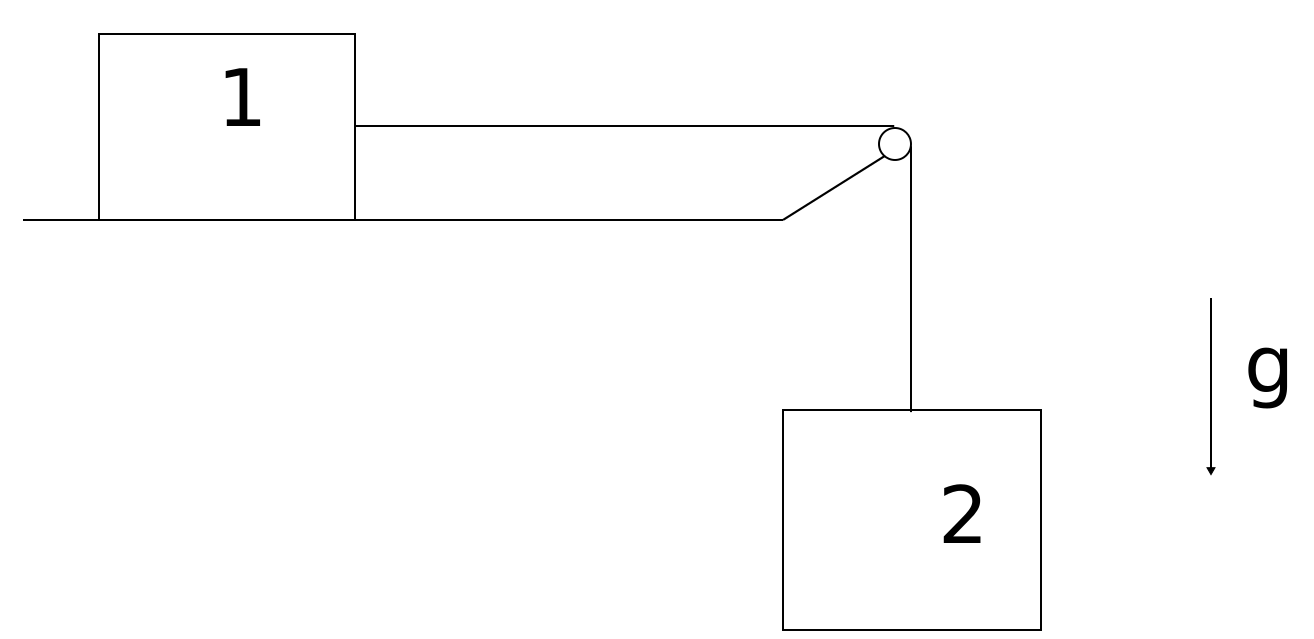
\includegraphics[width=.5\textwidth]{mult_lagrange}
        \caption{Blocos 1 e 2, unidos por um fio ideal}
        \label{fig:mult_lagrange}
    \end{figure}
    \FloatBarrier

    Considerando ainda que $L = T - V$, como será visto na
    \autoref{ssec:lagrange_hamilton}, temos os termos para a lagrangiana tal
    como especificados na \autoref{tab:lagrange_multipliers}, resultando na
    lagrangiana da \autoref{eq:eg_lag_mult}.

    \begin{table}[H]
        \centering
        \begin{tabularx}{\textwidth}{lllX}
            \toprule
            Origem & Coordenadas & Restrição & Termo da lagrangiana \\
            \midrule
            Bloco 1 & $x_1$, $y_1$ & -- & %
                $\frac{m_1}{2} \del{{\dot x_1}^2 + {\dot y_1}^2} - mgy_1$ \\
            Bloco 2 & $x_2$, $y_2$ & -- & %
                $\frac{m_2}{2} \del{{\dot x_2}^2 + {\dot y_2}^2} - mgy_2$ \\
            Mesa & $\lambda_1$ & $y_1 = 0$ & %
                $\lambda_1 \del{y_1 - 0}$ \\
            Fio & $\lambda_2$ & $x_1 + y_2 = -l$ &%
                $\lambda_2 \del{x_1 + y_2 + l}$ \\
            $\nexists~\text{movimento horizontal}$ & $\lambda_3$ & $x_2 = 0$ & %
                $\lambda_3 \del{x_2 - 0}$ \\
            \bottomrule
        \end{tabularx}
        \caption{Coordenadas e restrições dos multiplicadores de Lagrange}
        \label{tab:lagrange_multipliers}
    \end{table}
    
    \begin{equation}
        \label{eq:eg_lag_mult}
        L = \frac{m_1}{2} \del{{\dot x_1}^2 + {\dot y_1}^2} - m_1gy_1 + %
            \frac{m_2}{2} \del{{\dot x_2}^2 + {\dot y_2}^2} - m_2gy_2 + %
            \lambda_1 y_1 + %
            \lambda_2 \del{x_1 + y_2 + l} + %
            \lambda_3 x_2 
    \end{equation}
\end{eg}

Em resumo, uma restrição de coordenadas pode ser representada como $g(q_1,
\ldots, q_n, \dot q_1, \ldots, \dot q_n) = 0$. Se houver $k \in \mathbb{N}$
restrições em vigor em um determinado sistema, a lagrangiana modificada $L'$ que
incorpora essas restrições será dada por: 

\begin{equation}
    \label{eq:lag_mult}
    L' = L + \sum_{i=1}^{k} \lambda_i~g_i(q_1, \ldots, q_n, \dot q_1, \ldots, %
        \dot q_n)
\end{equation}

Onde $L$ é a lagrangiana original do sistema, e $\lambda_i$ são as coordenadas
extras que deverão ser levadas em consideração na resolução das equações de
Euler-Lagrange. 